\documentclass[10pt,a4paper]{article}

\usepackage{polski}
\usepackage[utf8]{inputenc}
\usepackage[T1]{fontenc}
\usepackage{amsmath,amssymb}
\usepackage{booktabs}
\usepackage{graphicx}
\usepackage{geometry}
\usepackage{microtype}
\usepackage{caption}
\usepackage{float}
\usepackage{tabularx}
\usepackage{titlesec}
\usepackage{enumitem}

\geometry{
    margin=1.6cm,
    top=1.4cm,
    bottom=1.4cm
}

\captionsetup{skip=2pt}
\titlespacing*{\section}{0pt}{4pt}{1pt}
\titlespacing*{\subsection}{0pt}{2pt}{1pt}
\setlength{\parskip}{1.5pt}
\setlength{\parindent}{0pt}
\setlist{nosep, leftmargin=12pt}

\title{\vspace{-1.0cm}\textbf{Obliczenia Naukowe - Lista 1}}
\author{Jakub Retmańczyk}
\date{25 października 2026}

\begin{document}

\maketitle
\vspace{-0.6cm}

\section{Zadanie 1}

Wyznaczyłem iteracyjnie epsilon maszynowy ($\text{macheps}$), najmniejszą dodatnią liczbę maszynową ($\eta$) oraz największą liczbę skończoną ($\text{MAX}$) dla typów \texttt{Float16}, \texttt{Float32} i \texttt{Float64}. Wyniki porównałem z funkcjami wbudowanymi Julii oraz wartościami z \texttt{float.h}.

\begin{table}[H]
\centering
\footnotesize
\caption{Porównanie parametrów arytmetyki wyznaczonych iteracyjnie ze stałymi bibliotecznymi.}
\label{tab:zad1}
\begin{tabularx}{\textwidth}{lXXX}
\toprule
\textbf{Parametr} & \textbf{Float16} & \textbf{Float32} & \textbf{Float64} \\
\midrule
$\text{macheps}$ (obliczone) & $9.765625 \cdot 10^{-4}$ & $1.19209290 \cdot 10^{-7}$ & $2.220446049250313 \cdot 10^{-16}$ \\
Wartość teoretyczna & $2^{-10}$ & $2^{-23}$ & $2^{-52}$ \\
\texttt{eps(T)} & $9.765625 \cdot 10^{-4}$ & $1.19209290 \cdot 10^{-7}$ & $2.220446049250313 \cdot 10^{-16}$ \\
\texttt{float.h} (\texttt{*\_EPSILON}) & - & $1.19209290 \cdot 10^{-7}$ & $2.220446049250313 \cdot 10^{-16}$ \\
\midrule
$\eta$ (obliczone) & $5.960464 \cdot 10^{-8}$ & $1.40129846 \cdot 10^{-45}$ & $4.940656458412465 \cdot 10^{-324}$ \\
Wartość teoretyczna & $2^{-24}$ & $2^{-149}$ & $2^{-1074}$ \\
\texttt{nextfloat(T(0.0))} & $5.960464 \cdot 10^{-8}$ & $1.40129846 \cdot 10^{-45}$ & $4.940656458412465 \cdot 10^{-324}$ \\
\midrule
\texttt{floatmin(T)} & $6.103516 \cdot 10^{-5}$ & $1.17549435 \cdot 10^{-38}$ & $2.225073858507201 \cdot 10^{-308}$ \\
Wartość teoretyczna & $2^{-14}$ & $2^{-126}$ & $2^{-1022}$ \\
\texttt{float.h} (\texttt{*\_MIN}) & - & $1.17549435 \cdot 10^{-38}$ & $2.225073858507201 \cdot 10^{-308}$ \\
\midrule
$\text{MAX}$ (obliczone) & $65504.0$ & $3.40282347 \cdot 10^{38}$ & $1.7976931348623157 \cdot 10^{308}$ \\
Wartość teoretyczna & $(2 - 2^{-10})\cdot 2^{15}$ & $(2 - 2^{-23})\cdot 2^{127}$ & $(2 - 2^{-52})\cdot 2^{1023}$ \\
\texttt{floatmax(T)} & $65504.0$ & $3.40282347 \cdot 10^{38}$ & $1.7976931348623157 \cdot 10^{308}$ \\
\texttt{float.h} (\texttt{*\_MAX}) & - & $3.40282347 \cdot 10^{38}$ & $1.7976931348623157 \cdot 10^{308}$ \\
\bottomrule
\end{tabularx}
\end{table}

\subsection*{Interpretacja}
\begin{itemize}
    \item Precyzja arytmetyki to połowa epsilona maszynowego: $\epsilon = \frac{1}{2}\text{macheps} = 2^{-t-1}$.
    \item Wartość $\eta$ to najmniejsza dodatnia liczba maszynowa większa od zera ($2^{e_{\min} - t}$, czyli $2^{-1074}$ w \texttt{Float64}), odpowiadająca \texttt{nextfloat(zero(T))}. Funkcja \texttt{floatmin} zwraca natomiast najmniejszą liczbę o pełnej precyzji mantysy ($2^{e_{\min}} = 2^{-1022}$). Zachodzi relacja $\eta = \text{macheps} \cdot \text{floatmin}$.
    \item Wyznaczone iteracyjnie parametry $\text{macheps}$, $\eta$ oraz $\text{MAX}$ są ściśle zgodne ze stałymi bibliotecznymi Julii oraz \texttt{float.h}.
\end{itemize}


\section{Zadanie 2}

Zbadałem, czy liczby \texttt{Float64} są równomiernie rozmieszczone w przedziale $[1, 2]$ z krokiem $\delta = 2^{-52}$ oraz jak wygląda rozmieszczenie w $[1/2, 1]$ i $[2, 4]$.

Dla każdego przedziału sprawdziłem $10^6$ kolejnych kroków \texttt{nextfloat}. Zależność $x = a + k \cdot \delta_a$ była spełniona w każdym kroku.

\begin{table}[H]
\centering
\small
\caption{Kroki siatki liczb maszynowych w badanych przedziałach (\texttt{Float64}).}
\label{tab:zad2_krok}
\begin{tabular}{lccc}
\toprule
\textbf{Przedział} & \textbf{Krok zmierzony $\delta_a$} & \textbf{Krok teoretyczny} & \textbf{Zgodność ($10^6$ kroków)} \\
\midrule
$[1/2, 1]$ & $\approx 1.110223 \cdot 10^{-16}$ & $2^{-53} = \frac{1}{2}\delta$ & Tak \\
$[1, 2]$   & $\approx 2.220446 \cdot 10^{-16}$ & $2^{-52} = \delta$            & Tak \\
$[2, 4]$   & $\approx 4.440892 \cdot 10^{-16}$ & $2^{-51} = 2\delta$           & Tak \\
\bottomrule
\end{tabular}
\end{table}

\begin{table}[H]
\centering
\footnotesize
\caption{Reprezentacja binarna liczb na granicach przedziałów (funkcja \texttt{bitstring}).}
\label{tab:zad2_bity}
\begin{tabular}{lccl}
\toprule
\textbf{Punkt $x$} & \textbf{Waga $2^p$} & \textbf{Format IEEE 754: znak $|$ cecha $|$ mantysa} & \textbf{Krok do sąsiada} \\
\midrule
$0.5$                   & $2^{-1}$ & \texttt{0 | 01111111110 | 0000\dots0000} & baza przedziału $[1/2, 1)$ \\
\texttt{nextfloat(0.5)} & $2^{-1}$ & \texttt{0 | 01111111110 | 0000\dots0001} & $+2^{-53} = \frac{1}{2}\delta$ \\
\midrule
$1.0$                   & $2^0$    & \texttt{0 | 01111111111 | 0000\dots0000} & nowa cecha ($1023$), baza $[1, 2)$ \\
\texttt{nextfloat(1.0)} & $2^0$    & \texttt{0 | 01111111111 | 0000\dots0001} & $+2^{-52} = \delta$ \\
$1.0 + 2\delta$         & $2^0$    & \texttt{0 | 01111111111 | 0000\dots0010} & $+2\cdot 2^{-52}$ \\
\midrule
$2.0$                   & $2^1$    & \texttt{0 | 10000000000 | 0000\dots0000} & nowa cecha ($1024$), baza $[2, 4)$ \\
\texttt{nextfloat(2.0)} & $2^1$    & \texttt{0 | 10000000000 | 0000\dots0001} & $+2^{-51} = 2\delta$ \\
\bottomrule
\end{tabular}
\end{table}

\subsection*{Interpretacja}
\begin{itemize}
    \item Liczby \texttt{Float64} są rozmieszczone lokalnie równomiernie w przedziałach $[2^p, 2^{p+1})$ ze stałym krokiem siatki $\delta_p = 2^{p-52}$.
    \item Każdą liczbę z przedziału $[2^p, 2^{p+1})$ można przedstawić jako $x = 2^p + k \cdot 2^{p-52}$ dla $k = 0, 1, \dots, 2^{52}-1$.
    \item Przekroczenie każdej kolejnej potęgi dwójki podwaja odległość między sąsiednimi liczbami maszynowymi.
\end{itemize}


\section{Zadanie 3}

Szukałem w arytmetyce \texttt{Float64} liczby $x \in (1, 2)$ takiej, że $\text{fl}(x \cdot \text{fl}(1/x)) \neq 1.0$.

\subsection*{Wyniki}
\begin{itemize}
    \item Zadanie 3a (dowolny przykład): już \texttt{nextfloat(1.5)} spełnia warunek:
    \begin{align*}
        x &= 1.5 + 2^{-52}, \quad
        \text{fl}(x \cdot \text{fl}(1/x)) = 1.0 - 2^{-53} \neq 1.0.
    \end{align*}
    \item Zadanie 3b (najmniejsza liczba): przeszukując od $1.0$ funkcją \texttt{nextfloat}, znalazłem ją po $257\,736\,490$ krokach:
    \begin{align*}
        x_{\min} &= 1.0 + 257\,736\,490 \cdot 2^{-52} \approx 1.00000005722899709681, \\
        \text{fl}(x_{\min} \cdot \text{fl}(1/x_{\min})) &= 1.0 - 2^{-53} \neq 1.0.
    \end{align*}
\end{itemize}

\subsection*{Pseudokod}
\begin{center}
\begin{minipage}{0.65\textwidth}
\hrule \vspace{2pt}
\footnotesize
Wyszukiwanie najmniejszego $x \in (1, 2)$ takiego, że $\text{fl}(x \cdot \text{fl}(1/x)) \neq 1$
\vspace{1pt}\hrule\vspace{2pt}
\begin{enumerate}
    \item $x \leftarrow \text{nextfloat}(1.0)$, \quad $k \leftarrow 1$
    \item \textbf{while} $x < 2.0$ \textbf{do}
    \item \quad \textbf{if} $x \cdot (1.0 / x) \neq 1.0$ \textbf{then return} $(x, k)$
    \item \quad $x \leftarrow \text{nextfloat}(x)$, \quad $k \leftarrow k + 1$
    \item \textbf{end while}
\end{enumerate}
\vspace{1pt}\hrule
\end{minipage}
\end{center}

\subsection*{Interpretacja}
Dla $x \in (1, 2)$ błąd zaokrąglenia odwrotności spełnia $x\delta < 2^{-53}$, co uniemożliwia zaokrąglenie iloczynu w górę; jedyną możliwą niezgodnością jest zaokrąglenie w dół do $1 - 2^{-53}$. Wymagany do tego margines błędu pojawia się po raz pierwszy dopiero przy kroku $k = 257\,736\,490$.


\section{Zadanie 4}

Obliczyłem iloczyn skalarny wektorów:
\begin{align*}
    x &= [2.718281828, -3.141592654, 1.414213562, 0.5772156649, 0.3010299957]^T, \\
    y &= [1486.2497, 878366.9879, -22.37492, 4773714.647, 0.000185049]^T,
\end{align*}
czterema metodami w precyzji \texttt{Float32} i \texttt{Float64}. Wartość dokładna: $S_{\text{dokładna}} = -1.00657107000000 \cdot 10^{-11}$.

\begin{table}[H]
\centering
\small
\setlength{\tabcolsep}{4.5pt}
\caption{Wyniki iloczynu skalarnego w arytmetyce \texttt{Float32} i \texttt{Float64}.}
\label{tab:zad4}
\begin{tabular}{lcccc}
\toprule
\textbf{Metoda} & \multicolumn{2}{c}{\textbf{Float32}} & \multicolumn{2}{c}{\textbf{Float64}} \\
\cmidrule(lr){2-3} \cmidrule(lr){4-5}
& Wartość & Błąd bezwzgl. & Wartość & Błąd bezwzgl. \\
\midrule
(a) w przód               & $-0.4999443$ & $0.4999443$ & $1.025 \cdot 10^{-10}$ & $1.126 \cdot 10^{-10}$ \\
(b) w tył                 & $-0.4543457$ & $0.4543457$ & $-1.564 \cdot 10^{-10}$ & $1.464 \cdot 10^{-10}$ \\
(c) od największych       & $-0.5000000$ & $0.5000000$ & $0.000000$                & $1.007 \cdot 10^{-11}$ \\
(d) od najmniejszych      & $-0.5000000$ & $0.5000000$ & $0.000000$                & $1.007 \cdot 10^{-11}$ \\
\bottomrule
\end{tabular}
\end{table}

\subsection*{Interpretacja}
\begin{itemize}
    \item Wynik iloczynu skalarnego ($10^{-11}$) powstaje z odejmowania składników rzędu $10^6$, powodując redukcję cyfr znaczących.
    \item Precyzja \texttt{Float32} (ok. 7 cyfr dziesiętnych) wyczerpuje się na samych składnikach rzędu $10^6$. Komputer traci część ułamkową i nie jest w stanie wyznaczyć różnicy rzędu $10^{-11}$ (stąd wynik ok. $-0.5$ i błąd względny rzędu $10^{10}$).
    \item W \texttt{Float64} metody (a) i (b) dają błąd względny ponad 1100\%. Metody (c) i (d) sumują składniki do dokładnie przeciwnych wartości maszynowych ($S_1 + S_2 = 0.0$); błąd bezwzględny wynosi wówczas $1.007 \cdot 10^{-11}$, lecz błąd względny to dokładnie 100\% (żadna cyfra znacząca nie jest poprawna).
\end{itemize}


\section{Zadanie 5}

Zbadałem wartości dwóch algebraicznie tożsamych funkcji dla $x = 8^{-k}$ ($k = 1, \dots, 25$):
\begin{equation}
    f(x) = \sqrt{x^2 + 1} - 1, \qquad g(x) = \frac{x^2}{\sqrt{x^2 + 1} + 1}.
\end{equation}

\begin{table}[H]
\centering
\small
\caption{Wartości $f(x)$ i $g(x)$ w arytmetyce \texttt{Float64}.}
\label{tab:zad5}
\begin{tabular}{rccc}
\toprule
$k$ & $x = 8^{-k}$ & $f(x)$ & $g(x)$ \\
\midrule
1  & $1.25 \cdot 10^{-1}$  & $7.782218537318641 \cdot 10^{-3}$  & $7.782218537318706 \cdot 10^{-3}$ \\
3  & $1.95 \cdot 10^{-3}$  & $1.907346813823096 \cdot 10^{-6}$  & $1.907346813826566 \cdot 10^{-6}$ \\
5  & $3.05 \cdot 10^{-5}$  & $4.656612873077393 \cdot 10^{-10}$ & $4.656612871993190 \cdot 10^{-10}$ \\
7  & $4.77 \cdot 10^{-7}$  & $1.136868377216160 \cdot 10^{-13}$ & $1.136868377216096 \cdot 10^{-13}$ \\
8  & $5.96 \cdot 10^{-8}$  & $1.776356839400250 \cdot 10^{-15}$ & $1.776356839400249 \cdot 10^{-15}$ \\
\textbf{9}  & $\mathbf{7.45 \cdot 10^{-9}}$  & $\mathbf{0.0}$ & $\mathbf{2.775557561562891 \cdot 10^{-17}}$ \\
10 & $9.31 \cdot 10^{-10}$ & $0.0$                & $4.336808689942018 \cdot 10^{-19}$ \\
15 & $2.84 \cdot 10^{-14}$ & $0.0$                & $4.038967834731580 \cdot 10^{-28}$ \\
20 & $8.67 \cdot 10^{-19}$ & $0.0$                & $3.761581922631320 \cdot 10^{-37}$ \\
\bottomrule
\end{tabular}
\end{table}

\begin{figure}[H]
\centering
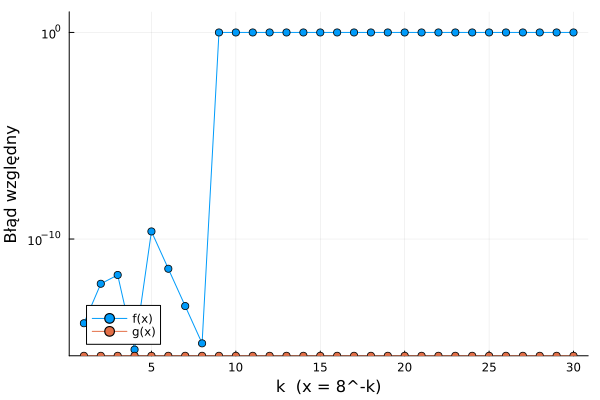
\includegraphics[width=0.36\textwidth]{zad5.png}
\caption{Porównanie wartości $f(x)$ i $g(x)$ w zależności od $k$.}
\label{fig:zad5}
\end{figure}

\subsection*{Interpretacja}
\begin{itemize}
    \item Wiarygodne są wyłącznie wyniki funkcji $g(x)$. We wzorze $f(x)$ od $k = 9$ wartość $x^2 \le 2^{-54}$ staje się mniejsza niż próg precyzji, więc komputer zaokrągla $x^2 + 1$ do $1.0$, dając błędne $f(x) = 0.0$.
    \item We wzorze $g(x)$ nie występuje odejmowanie bliskich sobie liczb, dlatego wyniki są poprawne dla wszystkich badanych $k$.
\end{itemize}


\section{Zadanie 6}

Obliczyłem przybliżenie pochodnej $f(x) = \sin x + \cos 3x$ w punkcie $x_0 = 1$ ilorazem różnicowym w przód:
\begin{equation}
    \tilde{f}'(x_0) = \frac{f(x_0 + h) - f(x_0)}{h}, \qquad h = 2^{-n},\ n = 0, 1, \dots, 54.
\end{equation}
Wartość dokładna: $f'(1) = \cos(1) - 3\sin(3) \approx 0.116942281688538$.

\begin{table}[H]
\centering
\small
\caption{Przybliżenia pochodnej i błędy bezwzględne dla wybranych $h = 2^{-n}$.}
\label{tab:zad6}
\begin{tabular}{rcccc}
\toprule
$n$ & $h = 2^{-n}$ & $1 + h$ & Przybliżenie $\tilde{f}'(1)$ & Błąd bezwzględny \\
\midrule
0  & $1.0$                 & $2.0000000000000000$ & $2.017989$ & $1.9010$ \\
5  & $3.125 \cdot 10^{-2}$ & $1.0312500000000000$ & $0.243443$ & $1.2650 \cdot 10^{-1}$ \\
10 & $9.766 \cdot 10^{-4}$ & $1.0009765625000000$ & $0.120882$ & $3.9402 \cdot 10^{-3}$ \\
20 & $9.537 \cdot 10^{-7}$ & $1.0000009536743164$ & $0.116946$ & $3.8473 \cdot 10^{-6}$ \\
\textbf{26} & $\mathbf{1.490 \cdot 10^{-8}}$ & $\mathbf{1.0000000149011612}$ & $\mathbf{0.11694234}$ & $\mathbf{5.70 \cdot 10^{-8}}$ \\
\textbf{27} & $\mathbf{7.451 \cdot 10^{-9}}$ & $\mathbf{1.0000000074505806}$ & $\mathbf{0.11694232}$ & $\mathbf{3.46 \cdot 10^{-8}}$ \\
\textbf{28} & $\mathbf{3.725 \cdot 10^{-9}}$ & $\mathbf{1.0000000037252903}$ & $\mathbf{0.11694229}$ & $\mathbf{4.80 \cdot 10^{-9}}$ \\
35 & $2.910 \cdot 10^{-11}$ & $1.0000000000291038$ & $0.11693954$ & $2.7370 \cdot 10^{-6}$ \\
50 & $8.882 \cdot 10^{-16}$ & $1.0000000000000009$ & $0.00000000$ & $1.1694 \cdot 10^{-1}$ \\
52 & $2.220 \cdot 10^{-16}$ & $1.0000000000000002$ & $-0.5000000$ & $6.1694 \cdot 10^{-1}$ \\
\textbf{53} & $\mathbf{1.110 \cdot 10^{-16}}$ & $\mathbf{1.0000000000000000}$ & $\mathbf{0.00000000}$ & $\mathbf{1.1694 \cdot 10^{-1}}$ \\
\bottomrule
\end{tabular}
\end{table}

\begin{figure}[H]
\centering
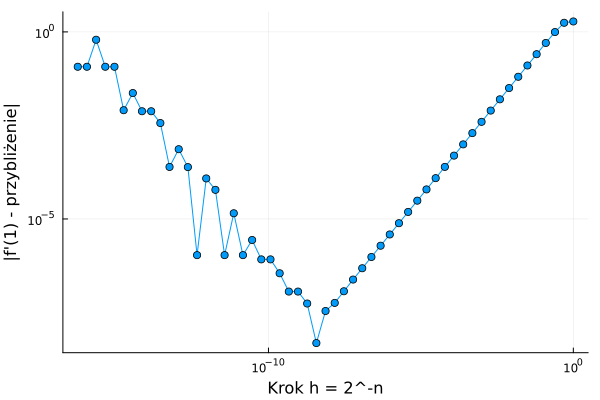
\includegraphics[width=0.33\textwidth]{zad6.png}
\caption{Błąd bezwzględny przybliżenia pochodnej w skali log-log.}
\label{fig:zad6}
\end{figure}

\subsection*{Interpretacja}
\begin{itemize}
    \item Błąd całkowity stanowi sumę błędu metody $O(h)$ (dominującego dla dużych $h$) oraz błędu zaokrągleń $O(\epsilon/h)$ (dominującego dla małych $h$).
    \item Optymalny krok minimalizujący błąd wynosi $h_{\text{opt}} \approx \sqrt{\text{macheps}} = 2^{-26} \approx 1.49 \cdot 10^{-8}$; najmniejszy błąd bezwzględny w eksperymencie uzyskałem dla $n = 28$ ($4.80 \cdot 10^{-9}$).
    \item Dla $n \ge 53$ zachodzi $\text{fl}(1+h) = 1.0$, przybliżenie pochodnej wynosi $0.0$, a błąd bezwzględny stabilizuje się na poziomie dokładnej wartości $|f'(1)| \approx 0.1169$ (błąd względny 100\%).
\end{itemize}

\end{document}
